\section{Experimental setup and results} \label{results}

\subsection{Data preparation}

To prepare a central dataset, both single datasets had to be transformed into a common format. For the central dataset only the class and the text content of each tweet respectively each forum contribution was considered.

The first dataset \citetitle{ThomasDavidson2020} was entirely given as a .csv file and contains 25.297 tweets, that were either labeled as hate speech, offensive language or neither of both. To determine the right label three independent evaluators classified each tweet, the final label got assigned by the majority vote. As for the first approach, one is only interested in hate speech and neutral tweet classification, all offensive language documents in the dataset were dropped. Some tweets were retweets that were commented additionally by a user. As it could not be distinguished whether the original tweet or the retweet contains hate speech, these documents were filtered out as well. An example is shown below:

\begin{quote}
    """@jaimescudi\_: ""@Tonybthrz\_: ""@jaimescudi\_: I swear if oomf try talking to me tomorrow.."" @"" @BarackObama"" pussy"
\end{quote}

The original tweets can be found in between the ""..."". Same goes for tweets that cite other users without using the retweet option.

\vspace{0.5cm}

The second dataset \citetitle{DeGibert2020} was not entirely given as a .csv file. Only the document annotations were given in a .csv file, all forum contributions were stored in separate .txt files. Only documents which could not be assigned to a single class (label "idk/skip") or referred to other documents (label "relation") were dropped.

The resulting common dataset was stored in a .csv file. It contains 2.491 hate speech documents and 13.336 non hate speech documents. The dropped offensive language documents make up 17.505 instances. In case the classification results are too poor, additional 2.818 offensive language documents can be added that were labeled as hate speech by one evaluator.

\subsection{Corpus building}

The common dataset is loaded from the .csv file into a pandas dataframe. After doing basic preprocessing like removing emojis and other irrelevant characters, spacy is used to build a tokenized corpus. The language model from spacy decides about stop word, punctuation and white space removal. No hard coded logic or stop word lists are used in this process. This keeps URLs or other tokens including punctuation as one token. Furthermore no stemming was applied to the tokens, instead lemmatization was used as one can in this case later on use pre-trained word embeddings from i.e. Word2Vec. Furthermore tokenization works better using the lemmas instead of word stems (e.g. We'll becomes ["we","will"] and not ["we", "'ll"].

Depending on the method the inputs vary. For the classical Machine Learning methods the inputs are the extracted features as numerical values, whereas in neural network based approaches the inputs are the raw textual features. The labels are in both cases numerical values.

Then we perform the dataset balancing. As already mentioned, the acquired dataset is an imbalanced one, which can lead to a decrease in performance and accuracy with machine learning classification. As a comparison the paper \cite{Oriola2020} also recognizes the class imbalance and tries to reduce it by applying a synthetic minority oversampling technique called SMOTE \cite{Chawla2011}. In general there are a few possibilities to tackle the challenge of unbalanced classes:

\begin{itemize}
    \item changing the performance metric (e.g. F1-score instead of accuracy)
    \item undersampling, i.e. deleting instances from the over-represented class
    \item oversampling, i.e. adding copies of instances from the under-represented class
    \item generating synthetic samples (e.g by using SMOTE)
\end{itemize}

In our experiments we chose to try the different approaches and applied a simple undersampling by randomly deleting instances from the over-represented class (neutral posts), as well as an oversampling using SMOTE. SMOTE does an oversampling by generating synthetic samples in the feature-space of the under-represented class, resulting in posts that statistically fall in between the different hate speech posts. Additionally, we used the imbalanced dataset to train a classifier to compare how this affects the performance.
Finally we receive unbalanced, undersampled and oversampled datasets, which we use for the further experiments. In addition for all experiments, we use the F1-score instead of the accuracy as our performance metric, which should somewhat handle unbalanced classes by itself.
Unfortunately, SMOTE only works in feature space, so we could not provide an oversampled balanced dataset for our neural network approach as this works directly on the hate speech and non-hate speech posts. This could be addressed in future work.

\subsection{Data analysis} \label{sec:data_analysis}

%TODO: Mit Hate Speech Statistics mergen?

In an in-depth analysis of the data, we had a look at the length of hate speech posts versus non-hate speech posts. This can be seen in \autoref{fig:post_length_density_distribution}.

\begin{figure}[ht]
    \centering
    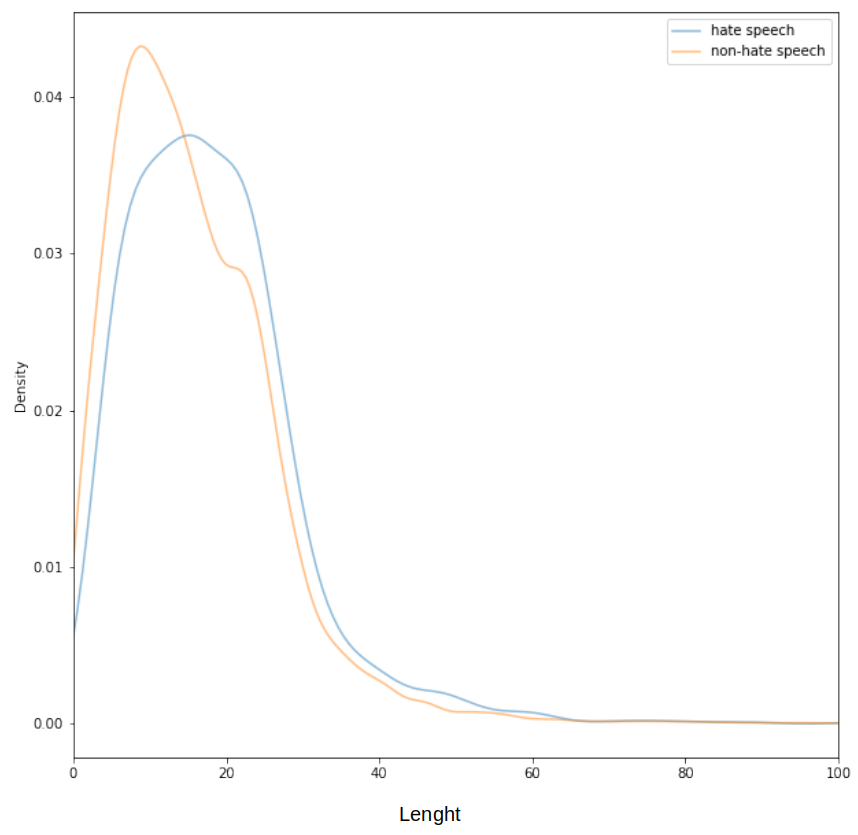
\includegraphics[width=0.8\linewidth]{figures/post_length_density_distribution.png}
    \caption{Density distribution of the length of a post (tweet or forum post)}
    \label{fig:post_length_density_distribution}
\end{figure}

Here one can see, that the hate speech posts contain more words (tokens before cleaning) than non-hate speech posts. In average a hate speech post contains 18.18 words, whereas a non-hate speech post only contains 15.85 words. Unlike expected, the hate speech posts are longer than the non-hate speech posts.

A more interesting look at the data is given by the most commonly used words per class. As can be seen in the word clouds in \autoref{fig:wordclouds} there are some obvious differences, such that the hate speech posts use words like \enquote{bitch}, \enquote{faggot} or \enquote{nigga}. But interestingly enough, the non-hate speech posts also sometimes consist of the words \enquote{trash} or \enquote{white}.

\begin{figure}[ht]
    \hfill
    \begin{subfigure}[b]{0.4\textwidth}
        \centering
        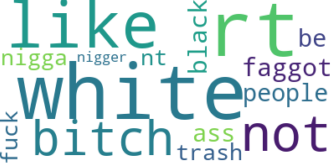
\includegraphics[width=\textwidth]{figures/Wordcloud-HateSpeech-tokens.png}
        \caption{hate speech}
    \end{subfigure}
    \hfill
    \begin{subfigure}[b]{0.4\textwidth}
        \centering
        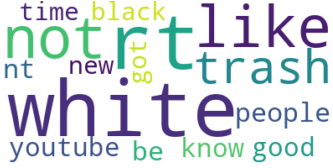
\includegraphics[width=\textwidth]{figures/Wordcloud-Non-HateSpeech-tokens.png}
        \caption{non-hate speech}
    \end{subfigure}
    \hfill
    \caption{Word clouds}
    \label{fig:wordclouds}
\end{figure}

For a better insight with what data we are dealing, a few examples are shown in the following.

\noindent
Examples for non-hate speech (neutral sentences):
\begin{itemize}
    \item "billy that guy wouldn't leave me alone so i gave him the trudeau salute"
    \item "this is after a famous incident of former prime minister pierre trudeau who gave the finger to a group of protesters who were yelling antifrench sayings at him"
    \item "askdems aren't you embarrassed that charlie rangel remains in your caucus"
\end{itemize}

\noindent
Examples for hate speech:
\begin{itemize}
    \item "california is full of white trash"
    \item "and yes they will steal anything from whites because they think whites owe them something so it's ok to steal"
    \item "why white people used to say that sex was a sin used to be a mystery to me until i saw the children of browns and mixed race children popping up all around me"
\end{itemize}

One can clearly see the hate expressed in the hate speech examples and see their discriminating nature.

\subsection{Experimental details}

%TODO: Hyperparameter vielleicht in den Anhang?

The optimal hyperparameters of the conventional Machine Learning methods are learned automatically as part of the pipeline. Nevertheless the learned optimal hyperparameters are listed in this chapter to enable the replication of our results. For readability only the hyperparameters, which differ from the default values are listed.

Optimal hyperparameters for the unbalanced dataset:
\begin{itemize}
	\item Decision Tree: max\_leaf\_nodes=15, min\_samples\_leaf=10
	\item Random Forest: criterion='entropy', max\_depth=10, max\_features='log2'
	\item SVM: kernel='linear'
	\item Logistic Regression: C=1.2, max\_iter=1500
\end{itemize}

Optimal hyperparameters for the undersampled dataset:
\begin{itemize}
	\item Decision Tree: class\_weight='balanced', criterion='entropy', max\_depth=10, max\_leaf\_nodes=15, min\_samples\_split=40
	\item Random Forest: max\_depth=10, max\_features='sqrt'
	\item SVM: kernel='linear'
	\item Logistic Regression: C=1.2, max\_iter=1500, solver='saga'
\end{itemize}

Optimal hyperparameters for the oversampled dataset:
\begin{itemize}
	\item Decision Tree: class\_weight='balanced', criterion='entropy'
	\item Random Forest: criterion='entropy', max\_features='sqrt'
	\item SVM: all default parameters
	\item Logistic Regression: C=1.2, max\_iter=1500
\end{itemize}

\subsection{Classifier metrics}
\label{ch:experimentDc}

Table \ref{Tab:unchanged} shows the performance metrics of the classifiers for the unbalanced dataset. 

\begin{table}[hbt!]
	\caption{Classifier results for unbalanced dataset}
	\label{Tab:unchanged}
	\begin{tabular}{|p{0.3\textwidth}|p{0.13\textwidth}|p{0.13\textwidth}|p{0.13\textwidth}|p{0.13\textwidth}|}
		\hline
		\textbf{classifier} & \textbf{precision} & \textbf{recall} & \textbf{accuracy} & \textbf{F1} \\ \hline
		Decision Tree       & \gradient{0.8756} & \gradient{0.9821} & \gradient{0.8671} & \gradient{0.9258} \\ \hline
		Random Forest       & \gradient{0.8809} & \gradient{0.9894} & \gradient{0.8782} & \gradient{0.9320} \\ \hline
		SVM                 & \gradient{0.8697} & \gradient{0.9927} & \gradient{0.8684} & \gradient{0.9272} \\ \hline
		Logistic Regression & \gradient{0.8831} & \gradient{0.9832} & \gradient{0.8760} & \gradient{0.9305} \\ \hline
		LSTM                & \gradient{0.9219} & \gradient{0.9567} & \gradient{0.8950} & \gradient{0.9390} \\ \hline
	\end{tabular}
\end{table}

\subsection{Oversampled and undersampled datasets}
\label{ch:experimentDd}

Table \ref{Tab:undersampled} shows the performance metrics of the classifiers for the undersampled dataset and table \ref{Tab:oversampled} for the oversampled dataset. 

\begin{table}[hbt!]
	\caption{Classifier results for undersampled dataset}
	\label{Tab:undersampled}
	\begin{tabular}{|p{0.3\textwidth}|p{0.13\textwidth}|p{0.13\textwidth}|p{0.13\textwidth}|p{0.13\textwidth}|}
		\hline
		\textbf{classifier} & \textbf{precision} & \textbf{recall} & \textbf{accuracy} & \textbf{F1} \\ \hline
		Decision Tree       & \gradient{0.7202} & \gradient{0.7710} & \gradient{0.7431} & \gradient{0.7448} \\ \hline
		Random Forest       & \gradient{0.7261} & \gradient{0.8043} & \gradient{0.7573} & \gradient{0.7632} \\ \hline
		SVM                 & \gradient{0.7193} & \gradient{0.8375} & \gradient{0.7621} & \gradient{0.7739} \\ \hline
		Logistic Regression & \gradient{0.7246} & \gradient{0.8238} & \gradient{0.7621} & \gradient{0.7710} \\ \hline
		LSTM                & \gradient{0.9219} & \gradient{0.9567} & \gradient{0.8950} & \gradient{0.9390} \\ \hline
	\end{tabular}
\end{table}

\begin{table}[hbt!]
	\caption{Classifier results for oversampled dataset}
	\label{Tab:oversampled}
	\begin{tabular}{|p{0.3\textwidth}|p{0.13\textwidth}|p{0.13\textwidth}|p{0.13\textwidth}|p{0.13\textwidth}|}
		\hline
		\textbf{classifier} & \textbf{precision} & \textbf{recall} & \textbf{accuracy} & \textbf{F1} \\ \hline
		Decision Tree       & \gradient{0.7973} & \gradient{0.7919} & \gradient{0.7924} & \gradient{0.7946} \\ \hline
		Random Forest       & \gradient{0.8844} & \gradient{0.8557} & \gradient{0.8701} & \gradient{0.8698} \\ \hline
		SVM                 & \gradient{0.7648} & \gradient{0.8081} & \gradient{0.7767} & \gradient{0.7859} \\ \hline
		Logistic Regression & \gradient{0.7573} & \gradient{0.8081} & \gradient{0.7713} & \gradient{0.7819} \\ \hline
		LSTM                & \multicolumn{4}{|c|}{not measured} \\ \hline
	\end{tabular}
\end{table}
